\begin{frame}{Avaliação de desempenho}
	\begin{itemize}
		\item A capacidade de um sistema computacional pode ser estimada mediante o emprego de técnicas de avaliação de desempenho.
		
		\item O método de \textbf{avaliação de desempenho} convencional em sistemas computacionais consiste em: 
		\begin{enumerate}
			\item Aplicar carga de interesse;
			\item Esperar estabilizar;
			\item Medir a saída.  
			\item<2> \textbf{Entrada vs. Saída} (extrair um modelo do sistema \textit{f(x)})
		\end{enumerate}
	\end{itemize}
	\note{com o objetivo de obter um modelo de desempenho quando comparado a entrada e a saída}
\end{frame}
	
\begin{frame}{Avaliação de desempenho estacionária}
	\note{note text}
	\begin{itemize}
		\item Na condição estacionária, os valores médios de entrada e saída não se alteram com o tempo; 
		\item O desempenho estacionário caracteriza-se por valores médios.  
		\begin{itemize}
			\item A análise procura determinar o valor médio da saída em função do valor médio da entrada.
		\end{itemize}
	\end{itemize}
	\begin{figure}
		\centering
		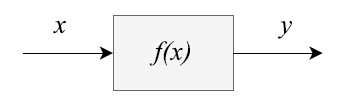
\includegraphics[scale=.6]{images/performance-1-pt.png}
		%\caption{Comportamento do serviço de um sistema computacional no tempo.}
		\label{fig:bloco-estacionario}
	\end{figure}
	\begin{block}{Saída em função da entrada}
		\begin{equation}
			y = f(x)
		\end{equation} 
	\end{block}
\end{frame}


\begin{frame}{Avaliação de desempenho estacionária}
	\begin{itemize}
		\item Sistemas que não possuem dinâmica (ou inércia) estão sempre na condição estacionária (caso de muitas aplicações em sistemas computacionais).  
		\item Por essa razão, a avaliação estacionária é predominante e não se fala muito em outro tipo de alternativa.
	\end{itemize}
\end{frame}

\begin{frame}{Sistemas com inercia}
	\begin{itemize}
		\item Quando o sistema possui inércia (ou dinâmica própria), contudo, uma mudança na entrada \underline{demora} um tempo para manifestar-se na saída. 
		\item Durante esse \underline{tempo}, mesmo sob uma carga constante na \underline{entrada}, o sistema pode apresentar uma \underline{saída} que varia com o tempo, conforme a perturbação se propaga.  
		\item Quando um sistema possui dinâmica, a análise estacionária não revela tudo sobre o sistema. 
	\end{itemize}
	
	\begin{figure}
		\centering
		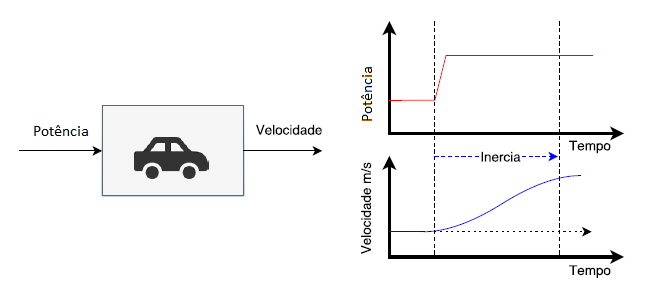
\includegraphics[scale=.4]{images/car-pt-crop.png}
		\caption{Inercia na aceleração do carro.}
		
	\end{figure}
\end{frame}

\begin{frame}{Transiente}	
	\begin{itemize}
		\item O tempo que a saída leva para ir de um patamar ao outro e se estabilizar é chamado de \textbf{transiente}.  
		\item A avaliação de desempenho não-estacionária objetiva estudar tanto o estado \underline{transiente} quanto o \underline{estacionário} (engloba a estacionária).
	\end{itemize}
	\begin{figure}
		\centering
		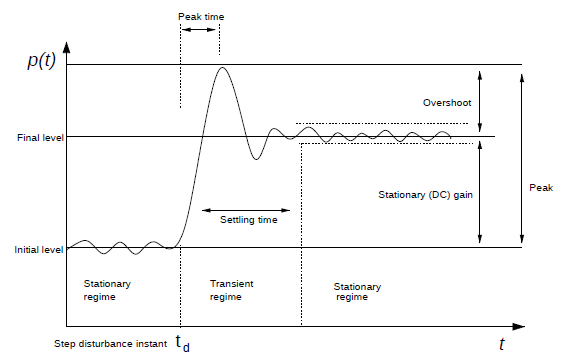
\includegraphics[scale=.4]{images/dynamics.png}
		\caption{Comportamento de um sistema computacional no tempo.}
		\label{fig:respota-vs-tempo}
	\end{figure}	
\end{frame}


\begin{frame}{Contextualização}
	\begin{columns}
		\column{0.35\textwidth}
		\begin{minipage}[c][0.25\textheight][c]{\linewidth}
			\begin{itemize}
				\item Com o crescimento das aplicações intensivas de dados, a dinâmica do sistema passa ser apreciável, tais aplicações tendem a operarem com cargas de trabalho variante no	tempo, causando inúmeras dificuldades \cite{Padala2007}; 				
			\end{itemize}
		\end{minipage}
		\column{0.6\textwidth}
		\begin{minipage}[c][0.4\textheight][c]{\linewidth}
			\centering
			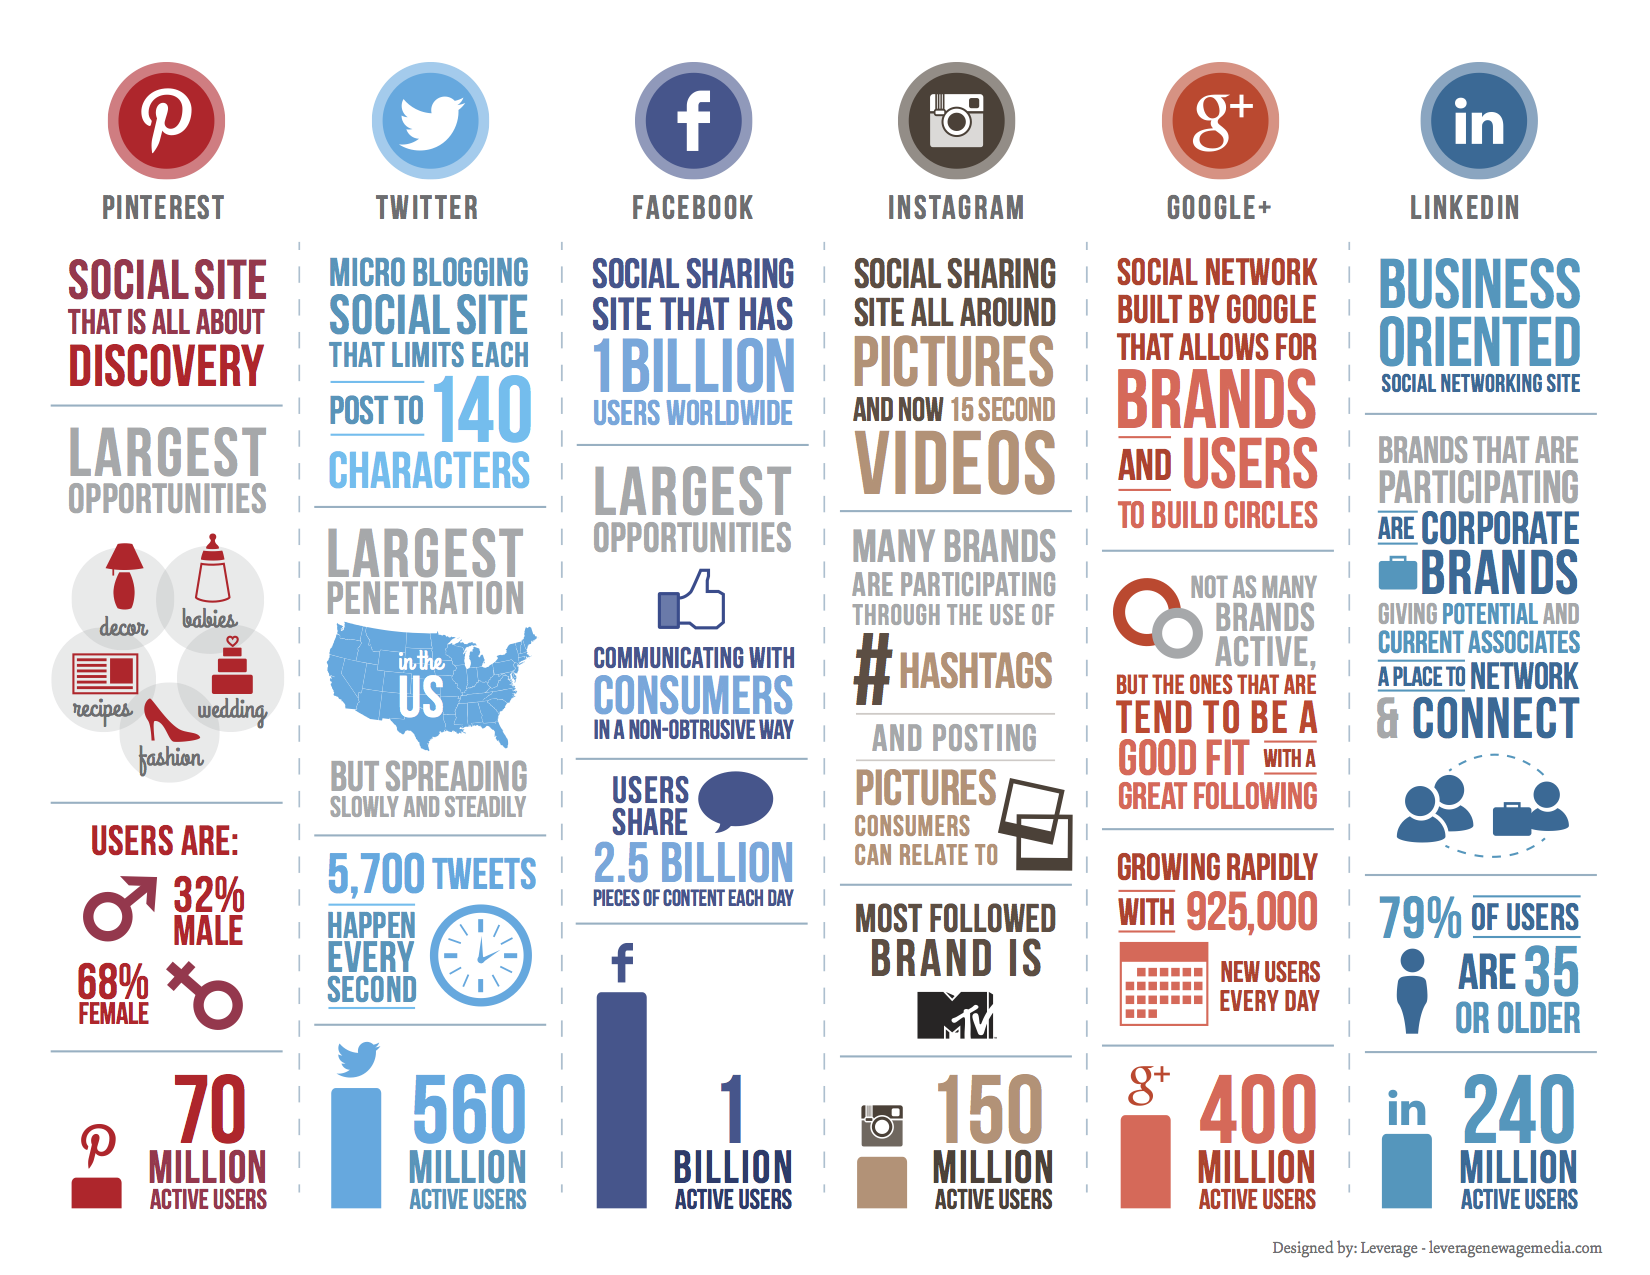
\includegraphics[scale=0.27]{images/social-media-networks.png}
		\end{minipage}		
	\end{columns}	
\end{frame}


\begin{frame}{Dinâmica de primeira ordem em um sistema físico}
	\begin{figure}[htb]
		\centering
		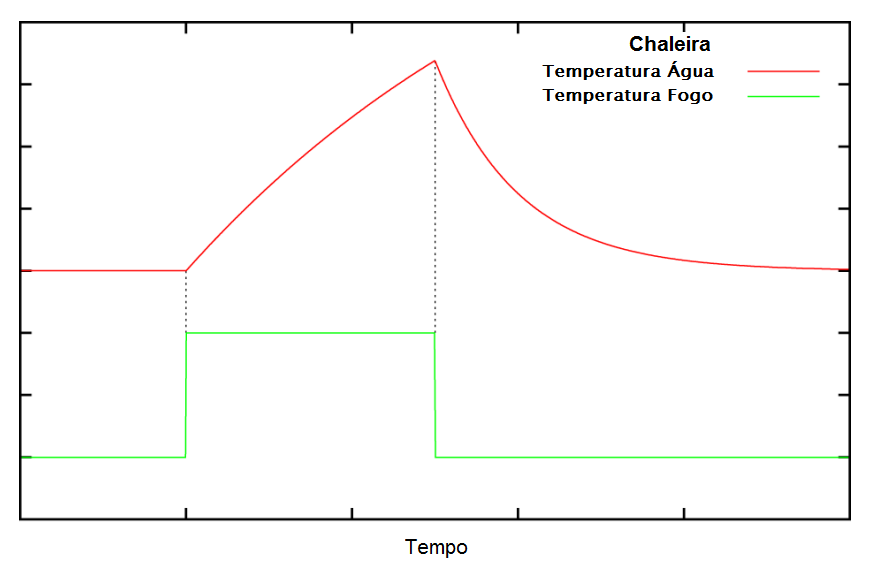
\includegraphics[scale=0.4]{../monograph/images/grafico-chaleira.png}	
		\caption{Dinâmica da chaleira aquecendo \cite{Janert2013}}
	\end{figure}
\end{frame}

\begin{frame}{Dinâmica de primeira ordem em um sistema computacional}
	\begin{figure}[htb]
		\centering
		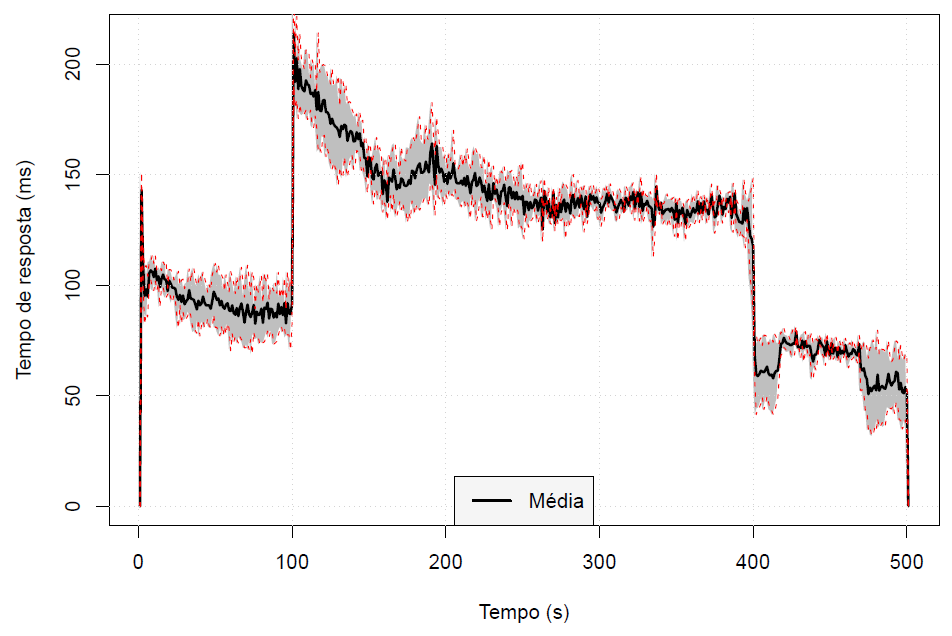
\includegraphics[scale=0.4]{images/tempo-resposta-db2-crop.png}	
		\caption{Dinâmica em banco de dados \cite{Edwin2015}}
	\end{figure}
\end{frame}

\begin{frame}{Dinâmica de segunda ordem em sistema físico}
	\begin{figure}[htb]
		\centering
		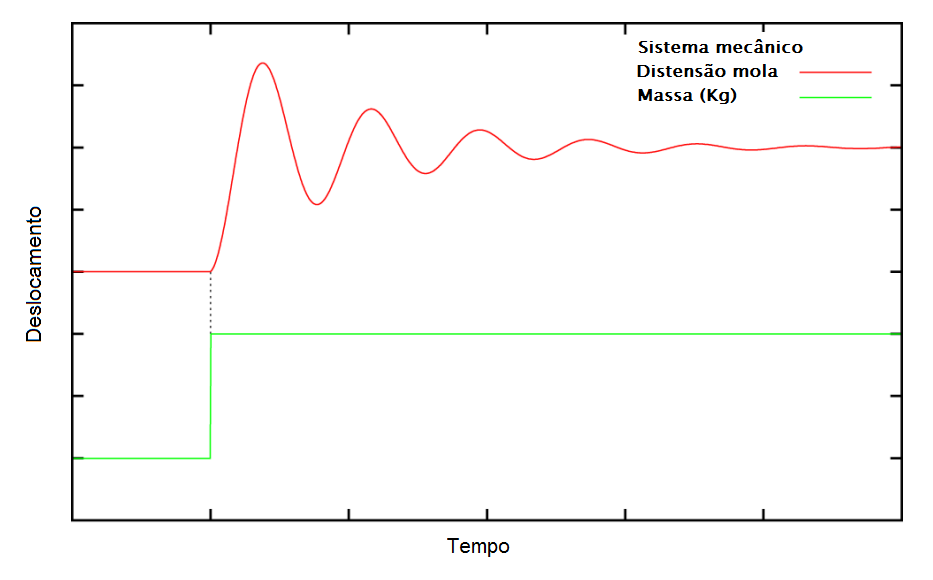
\includegraphics[scale=0.4]{../monograph/images/grafico-mola.png}	
		\caption{Dinâmica da mola \cite{Janert2013}}
	\end{figure}
\end{frame}

\begin{frame}{Dinâmica de segunda ordem em sistema computacional}
	\begin{figure}
		\centering
		\begin{minipage}{.45\textwidth}
			\centering
			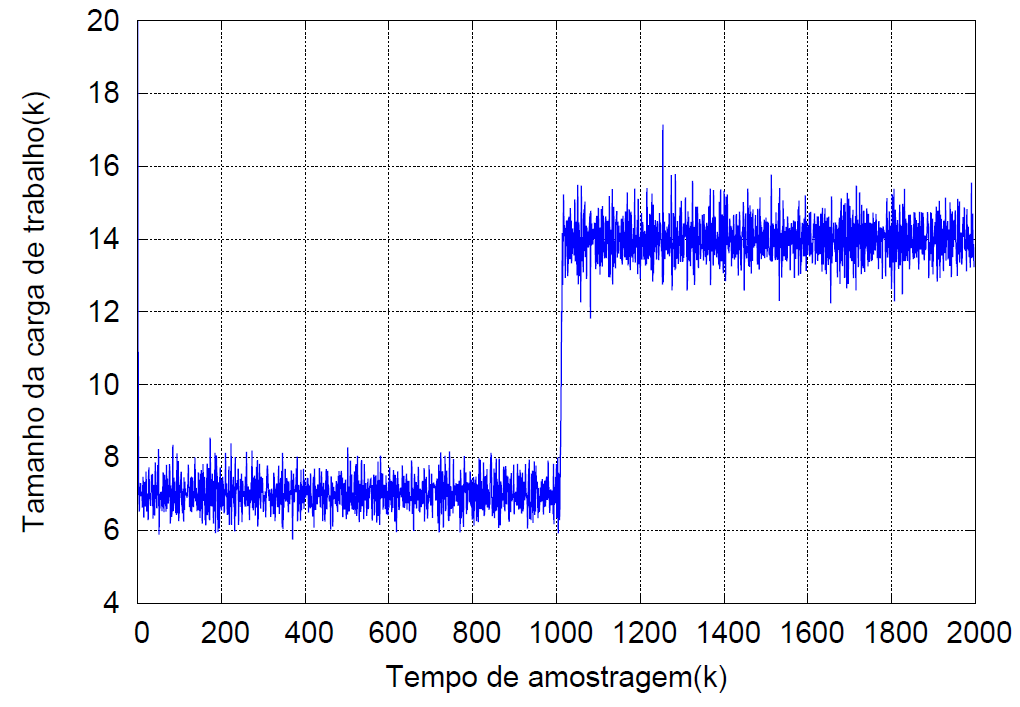
\includegraphics[scale=0.2]{images/entrada_resultado_helder_sys_segunda_orderm.png}	
			%\caption{A subfigure}
		\end{minipage}
		\begin{minipage}{.45\textwidth}
			\centering
			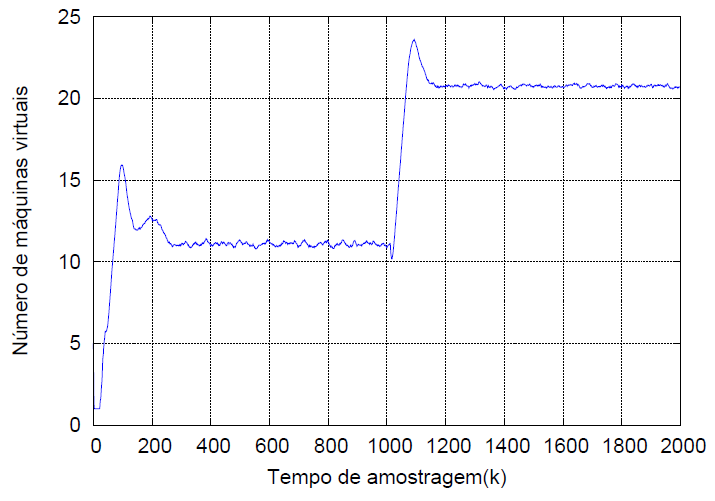
\includegraphics[scale=0.29]{images/resultado_helder_sys_segunda_orderm.png}	
			%\caption{A subfigure}
		\end{minipage}
		\caption{Dinâmica de controlador \cite{helder2014}}
	\end{figure}
%	\begin{figure}
%		\begin{minipage}{.5\textwidth}
%			\centering
%			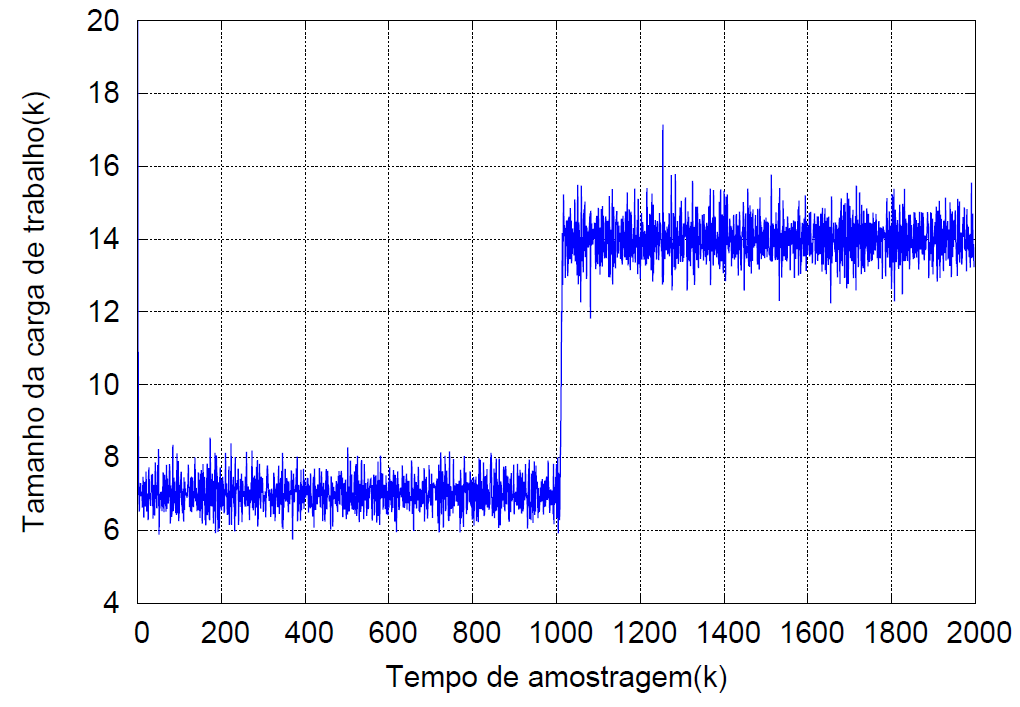
\includegraphics[scale=0.22]{images/entrada_resultado_helder_sys_segunda_orderm.png}	
%			\caption{A subfigure}
%		\end{minipage}
%		\begin{minipage}{.5\textwidth}
%			\centering
%			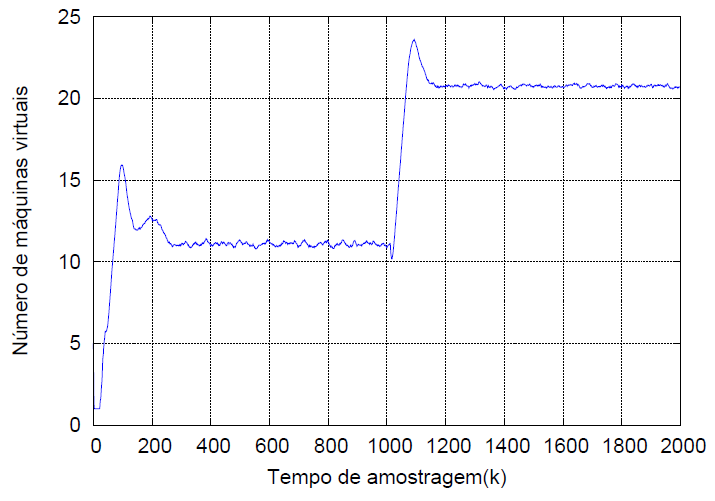
\includegraphics[scale=0.31]{images/resultado_helder_sys_segunda_orderm.png}	
%			\caption{A subfigure}
%		\end{minipage}
%		\caption{Dinâmica de controlador \cite{helder2014}}
%	\end{figure}	
\end{frame}

\begin{frame}{Avaliação de desempenho não-estacionária}
	\begin{itemize}
		\item O interesse da computação vem aumentando. \textbf{Por quê?}
		\item A avaliação estacionária procura determinar o valor médio do desempenho ao longo de um intervalo de operação
		\item A avaliação não-estacionária ou \textbf{transiente}, busca determinar \underline{como} o valor instantâneo do desempenho \textbf{varia com o tempo}.  
	\end{itemize}
	\begin{figure}
		\centering
		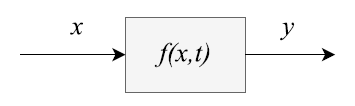
\includegraphics[scale=.6]{images/performance-2-pt.png}
		%\caption{Comportamento do serviço de um sistema computacional no tempo.}
		\label{fig:bloco-nao-estacionario}
	\end{figure}
	\begin{block}{Saída em função da entrada e do tempo}
		\begin{equation}
		y = f(x,t)
		\end{equation} 
	\end{block}
	\note{A diferença aqui é que estamos dizendo que a saída y depende da entrada e também do tempo. Nesse caso t aparece como variável independente de x.  Isso quer dize que mesmo com x constante, y pode variar. E a variação de y com x constante é devido ás mudanças no estado interno do sistema. Um sistema dinâmico possui estados internos. Um sistema que não é dinâmico não possui estados internos, e por isso, a saída é determinada unicamente pela entrada.  Entenda isso, Edwin. É muito importante. Se você me diz que a pressão atualmente aplicada ao acelerador do carro é x, eu não sei qual a velocidade y apenas com essa informação. Eu precisaria perguntar pra você qual a velocidade inicial do carro e por quanto tempo você está mantendo a pressão no acelerador.  Isso porque o carro é um sistema dinâmico; a velocidade vai aumentando mesmo que a pressão no acelerador seja constante.}
\end{frame}



\begin{frame}{Motivação}
	Esse problema vem sendo estudando no grupo de pesquisa e foi pesquisado na área de simulação, sendo uma das contribuições:
	\begin{itemize}
		\item Um modelo conceitual de requisitos denominado MEDC \cite{Lourenco2015}
	\end{itemize}
	%Un modelo conceitual de requisitos denominado MEDC
\end{frame}

\begin{frame}{Objetivo de pesquisa do trabalho vinculado}	
	\begin{block}{}{
			O objetivo de \cite{Edwin2015} é formular uma metodologia para projeto de \textit{benchmarks} para avaliação de desempenho não-estacionaria de sistemas computacionais baseado no modelo de aspectos MEDC. 
		}
		\begin{itemize}
			\item Contribuições:
			\begin{itemize}
				\item Demostra que a metodologia abstrata MEDC proposta originalmente para simulação, é aplicável também a problemas de \textit{benchmarks}, bem como ela pode ser instanciada nesse outro domínio.
			\end{itemize}
		\end{itemize}
	\end{block}
	\label{section:intro-goal}
	
	\note{* Uma das contribuições pretendidas pela nossa pesquisa é evidenciar quando a avaliação de desempenho não estacionária é importante em sistemas computacionais.  Por exemplo, é interessante em sistemas de grande escala e sistemas multicamadas, onde a interação entre as partes pode resultar em propriedades dinâmicas apreciáveis. Em trabalhos anteriores temos discutido isso em sistemas de computação em nuvem, por exemplo.
		
		* Na nossa investigação observamos que a maioria dos benchmarks são projetados para avaliação estacionária e não atendem os requisitos necessários para realização de experimentos com a finalidade de fazer a avaliação dinâmica.  Um desses requisitos é a incapacidade de modulação de demanda. Para se obter informações sobre o estado transiente, é preciso provocar esse transiente no sistema. Isso se faz aplicando uma perturbação na entrada, a qual tire o sistema do estacionário e exponha os efeitos transitórios.  Os benchmarks estudados não possuem recursos para isso.  Outra característica dos benchmarks convencionais é que eles fornecem medidas agregadas, por exemplos valores médios obtidos durante o experimento.  Em avaliação dinâmica precisamos dos valores ao longo do tempo.
		
		* Com base nessas limitações, procuramos elicitar requisitos específicos que um framework de benchmark deve atender para que seja útil em avaliação dinâmica.  
		
		* Em uma pesquisa em desenvolvimento no grupo, um trabalho anterior fez esse estudo no contexto de simulação de eventos discretos para avaliação de desempenho não estacionária em sistemas computacionais.  O trabalho propôs um modelo conceitual de separação de responsabilidades que foi denominado MEDC.}
\end{frame}

\begin{frame}{Objetivo}
	\begin{block}{}{
			A extensão do \textit{framework} de \textit{benchmark} Bench4Q a fim de atender um dos requisitos do modelo MEDC. 
		}
		\begin{itemize}					
			\item Restringe-se ao requisito de modulação da carga de trabalho, gerado pelo \textit{benchmark}, correspondente ao modulo \textit{Demand} do MEDC
			
			\item A contribuição almejada é a disponibilização de um \textit{benchmark} que auxilie a análise de sistemas dinâmicos e que possibilite a análise transiente.
		\end{itemize}
	\end{block}	
\end{frame}	